\chapter{Literature review}

\section{Basic aviation terminologies}

\subsection{UAV or Drone}
UAV is short for Unmanned Aerial Vehicle, in other words an airborne vehicle that is capable of movement
without having a pilot on board. Drone is a subset of UAV, a vehicle that is capable of autonomous flight.
Usually UAV and the word Drone are used interchangeably in the literature, and it is used so in this thesis.

\subsection{Body axes used in aviation}
In aviation Euler angles are used to describe the orientation of an aircraft. Euler angles are three angles
that describe the orientation of a rigid body with respect to a fixed coordinate system. These axes are 
referred to as Yaw, Pitch and Roll. Rotation around these axes are Yaw, Pitch 
and Roll angles respectively. All three angles follow the right-hand rule. 

Magnetic north is used as reference for Yaw, so an angle of 0$^\circ$ or 360$^\circ$ means that the vehicle
is heading North, 90$^\circ$ means it's heading East. Yaw is sometimes called Heading.

\begin{figure}[!hb]
    \centering
	$\vcenter{\hbox{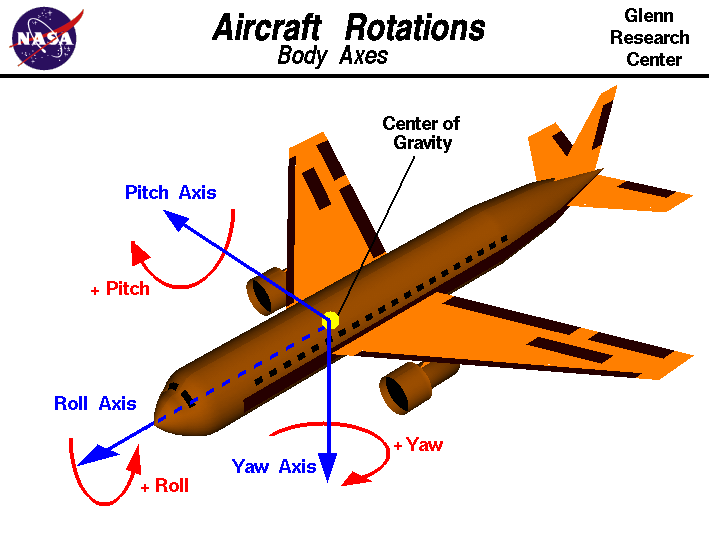
\includegraphics[width=90mm, keepaspectratio]{figures/plane_yaw_pitch_roll.png}}}$
    $\vcenter{\hbox{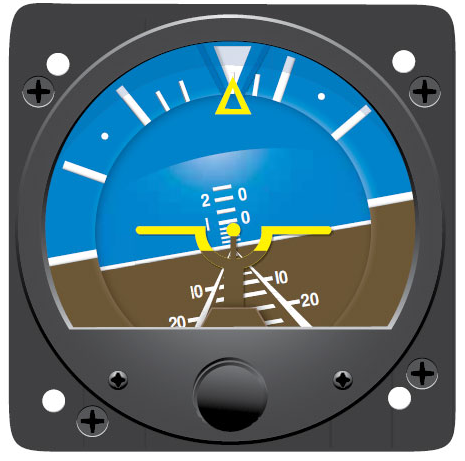
\includegraphics[width=40mm, keepaspectratio]{figures/attitude_indicator.png}}}$
    \caption{Aircraft body axes\cite{AircraftBodyAxes} and attitude instrument}
    \label{fig:aircraft_body_angles}
\end{figure}


Pitch and Roll angles are calculated in reference to the horizontal plane. The normal vector of the horizontal 
plane is used for the calculations, and it is the norm of the gravity vector. It is favorable to use the gravity
vector, because its direction can be measured using an accelerometer. Both Roll and Pitch angles are measured
from -90$^\circ$ to 90$^\circ$. A Pitch of 90$^\circ$ is straight up and 0$^\circ$ is Horizon. If an aircraft
flies with 0$^\circ$ Roll angle, the vehicle is horizontal. On the other hand a 90$^\circ$ Roll angle means
the vehicle is turning right and is perpendicular to the horizon. Pitch is sometimes referred to as Tilt.

The limitation of using Euler angles is reached when Pitch or Roll angles approach 90$^\circ$, because in this 
case one of these angles become parallel with the gravity vector and the other angle cannot be determined, 
due to lack of reference.
Euler angles and singularities are well described in \cite{diebel2006representing}. To avoid singularities
of Euler angles, Unit quaternions can be used. Quaternions are mainly used for calculations, while Euler 
angles are used to provide humanly readable values.

\subsection{Ground Control Station}
A software running on a ground computer, used for receiving in-flight information via telemetry from a UAV.
It displays status and progress of mission, that often includes sensor or video data. It can also be used
for sending commands up to the UAV during flight.

Ground Control Station is often referred to as GCS.

\subsection{Multicopters}
Multicopter or Multirotor is a generic term to describe a UAV with more than two rotors. The term covers quadcopters,
octocopters, hexicopters etc.

Quadcopters are quickly gaining popularity thanks to the easy to use, commercially available drones that can be used
for filming. Octocopters have eight rotors in total and mostly used by professional users. It provides a more stable 
flight, can lift more weight and it is safer, because it can fly with any of the rotors damaged.

\section{Simultaneous Localization And Mapping - SLAM}
Simultaneous Localization And Mapping the computational problem that asks if it is possible to place a robot 
in an unknown environment and for the robot to incrementally build a consistent map of this environment while 
simultaneously determining its position. A good overview of SLAM is presented in\cite{durrant2006simultaneous} 
and \cite{diebel2006representing} focusing a solution to the above proposed problem in general, with no dependency 
of sensors to be used.

\begin{figure}[!ht]
    \centering
	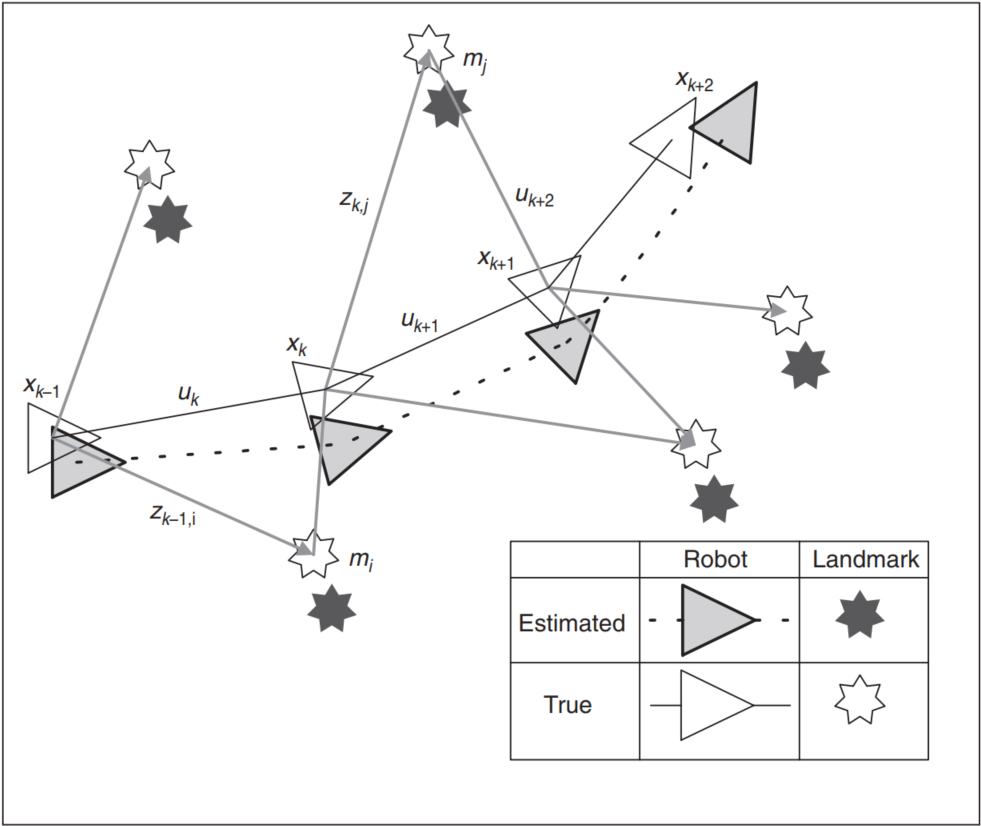
\includegraphics[width=80mm, keepaspectratio]{figures/slam_tutorial_basic_figure.png}
    \caption{The essential SLAM problem presented in \cite{durrant2006simultaneous} }
    \label{fig:slam_tutorial_basic}
\end{figure}

During SLAM process a robot is placed in an unknown location and it is capable of estimating its trajectory and 
location of all landmarks online, without the need of priori knowledge of the location. The robot makes relative
observations of its surroundings, a number of unknown landmarks using sensors as seen on figure \ref{fig:slam_tutorial_basic}.
The following quantities are defined at a time instant \emph{k}:
\begin{itemize}
	\item $\mathbf{x}_{k}$: State vector describing the location and orientation of the robot
	\item $\mathbf{u}_{k}$: Control vector, applied at \emph{k-1} and drove the robot to state $\mathbf{x}_{k}$ at time \emph{k}
	\item $\mathbf{m}_i$: Landmark location vector. A time independent vector that describes the location of a static landmark
	\item $\mathbf{z}_{ik}$: Observation taken from the robot to the \emph{i}th landmark at time \emph{k}
	\item $\mathbf{X}_{0:k}=\left \{ \mathbf{x}_1,\mathbf{x}_2,\cdots,\mathbf{x}_k \right \}$ A set of all robot location vectors until time \emph{k}
	\item $\mathbf{U}_{0:k}=\left \{ \mathbf{u}_1,\mathbf{u}_2,\cdots,\mathbf{u}_k \right \}$ A set of history of all control vectors until time \emph{k}
	\item $\mathbf{m}=\left \{ \mathbf{m}_1,\mathbf{m}_2,\cdots,\mathbf{m}_n \right \}$ A set of all landmarks
	\item $\mathbf{Z}_{0:k}=\left \{ \mathbf{z}_1,\mathbf{z}_2,\cdots,\mathbf{z}_k \right \}$: A set of all landmark observations until time \emph{k}
\end{itemize}

In probabilistic form of SLAM, the probability distribution function \ref{eq:slam_probability} needs to be computed for
all times \emph{k}. In other words the current state vector and the landmark location probabilities need to be calculated
based on all \emph{k} observations, control vectors and the initial state of the robot.

\begin{equation} \label{eq:slam_probability}
    P\left ( \mathbf{x}_{k},\mathbf{m}\mid \mathbf{Z}_{0:k},\mathbf{U}_{0:k},\mathbf{x}_{0}\right )
\end{equation}

A recursive solution is desirable for the SLAM problem. Starting with an estimate for the posteriori distribution 
(equation \ref{eq:slam_probability_posteriori}) at time \emph{k}-1, then a control vector $\mathbf{u}_{k}$ is used to
estimate the next state and observations using Bayes theorem. This calculation requires an observation model and a 
state transition model.
 


\begin{equation} \label{eq:slam_probability_posteriori}
    P\left ( \mathbf{x}_{k-1},\mathbf{m}\mid \mathbf{Z}_{0:k-1},\mathbf{U}_{0:k-1},\mathbf{x}_{0}\right )
\end{equation}

The observation model \ref{eq:slam_observation_model} describes the probability of making an observation 
$\mathbf{z}_{k}$ given the current robot and landmark locations.

\begin{equation} \label{eq:slam_observation_model}
    P\left ( \mathbf{z}_{k}\mid \mathbf{x}_{k},\mathbf{m} \right )
\end{equation}

The state transition model \ref{eq:slam_motion_model} describes the probability of the next position of the robot 
based on the previous state and the control vector at time \emph{k}. The state transition is assumed to be a Markov
process, so the next state $\mathbf{x}_{k}$ depends only on the current state $\mathbf{x}_{k-1}$ applied control 
$\mathbf{u}_{k}$. $\mathbf{x}_{k}$ is also independent from both landmark locations $\mathbf{m}$ and observations
$\mathbf{z}_{k}$.

\begin{equation} \label{eq:slam_motion_model}
    P\left ( \mathbf{x}_{k}\mid \mathbf{x}_{k-1},\mathbf{u}_{k} \right )
\end{equation}

Using equations \ref{eq:slam_probability_posteriori}, \ref{eq:slam_observation_model} and \ref{eq:slam_motion_model},
the SLAM algorithm can now be described using a two-step recursive form: prediction and correction.
The prediction step or time-update is used for estimating the next state and map, based on all posteriori observations,
control vectors and initial state. 

\begin{equation} \label{eq:slam_time_update}
    P\left ( \mathbf{x}_{k}, \mathbf{m}\mid \mathbf{Z}_{0:k-1}, \mathbf{U}_{0:k}, \mathbf{x}_{0} \right )=
        \int 
            P\left ( \mathbf{x}_{k}\mid \mathbf{x}_{k-1}, \mathbf{u}_{k} \right ) 
            \times  
            P\left ( \mathbf{x}_{k-1}, \mathbf{m}  \mid  \mathbf{Z}_{0:k-1}, \mathbf{U}_{0:k-1}, \mathbf{x}_{0}\right )
        d\mathbf{x}_{k-1}
\end{equation}

The measurement update provides a correction to the prediction state, using observations made at time \emph{k}.

\begin{equation} \label{eq:slam_mesurement_update}
    P\left ( \mathbf{x}_{k}, \mathbf{m} \mid \mathbf{Z}_{0:k}, \mathbf{U}_{0:k}, \mathbf{x}_{0} \right )= 
    \frac
        {P\left ( \mathbf{z}_{k}\mid \mathbf{x}_{k}, \mathbf{m} \right )P\left ( \mathbf{x}_{k}, \mathbf{m}\mid \mathbf{Z}_{0:k-1}, \mathbf{U}_{0:k}, \mathbf{x}_{0}\right ) }
        {P\left ( \mathbf{z}_{k} \mid \mathbf{Z}_{0:k-1}, \mathbf{U}_{0:k}\right )}
\end{equation}


The localization problem can be solved with the assumption the map is known:

\begin{equation} \label{eq:slam_localization_problem}
    P\left ( \mathbf{x}_{k} \mid \mathbf{Z}_{0:k}, \mathbf{U}_{0:k}, \mathbf{m}\right )
\end{equation}

And the mapping problem can be solved with the assumption the location is known:

\begin{equation} \label{eq:slam_mapping_problem}
    P\left ( \mathbf{m} \mid \mathbf{X}_{0:k}, \mathbf{Z}_{0:k}, \mathbf{U}_{0:k}, \right )
\end{equation}

These problems introduced in \ref{eq:slam_localization_problem} and \ref{eq:slam_mapping_problem} are
dependent on each other and need to be solves simultaneously. In the early stages of SLAM mapping and localization
were tried to be solved independently and work often focused on either of them. Once the realization came that combined 
mapping and localization can be formulated as a single estimation problem, the problem became convergent.

Many solutions can be found for probabilistic SLAM problem, the most common is the use of the extended Kalman
filter (EKF) that provides an optimal estimation to non-linear models with additive Gaussian noise. The motion
model can also be represented with a non-Gaussian probability distribution, that leads to the use of the 
Rao-Blackwellized particle filter, or FastSLAM algorithms.


The above introduced SLAM problem was a general introduction, it is not dependent on the sensor used for observations.
Many kind of observers can be used for this purpose, but the two main categories are visual or camera based and sensor based.
Visual observers mostly use simple or special camera configurations for depth sensing, while sensor based observers 
use some other technique or physical phenomena to measure distances like sonars or LIDARS.

\subsection{Visual SLAM}
Visual SLAM is a subset of SLAM algorithms that processes camera images to determine the camera's position and orientation
relative to its surroundings, while building a map of its environment. In the simplest case a monocular camera is used
to collect images, but more advanced active or passive stereo cameras and RGB-D cameras are also used. A pro of using
images for SLAM is that images contain high amounts of data, therefore very detailed maps can be made. On the other hand,
processing big amounts of data means higher complexity and demands higher processing capabilities.


Two main categories of visual techniques are feature-based and direct SLAM algorithms. Feature-based techniques detect
certain key-points called features in images, like corners and edges, and only use these features to extract depth information.
Direct SLAM algorithms however don't search for features, but use the image intensities to estimate the location and surroundings.
Two popular visual SLAM methods are feature-based ORB-SLAM and direct LSD-SLAM.

\subsubsection{Monocular camera}
The pro of using monocular camera for localization and mapping is that each image contains high density of information and
cameras will always be cheaper easier to use than other depth sensing camera rigs. 
A big pro, but in the same time a big con of using a monocular camera for SLAM is that a single camera cannot detect the scale.
It is an advantage, because the same camera can be used indoor on a small scale even down to centimeters, and used outdoors on
a scale of kilometers. Nonetheless these during transmission between these scales, the scale can drift and therefore size of
landmarks will not be presented correctly. This is called scale-drift, that algorithms try to compensate.

\begin{figure}[!ht]
    \centering
	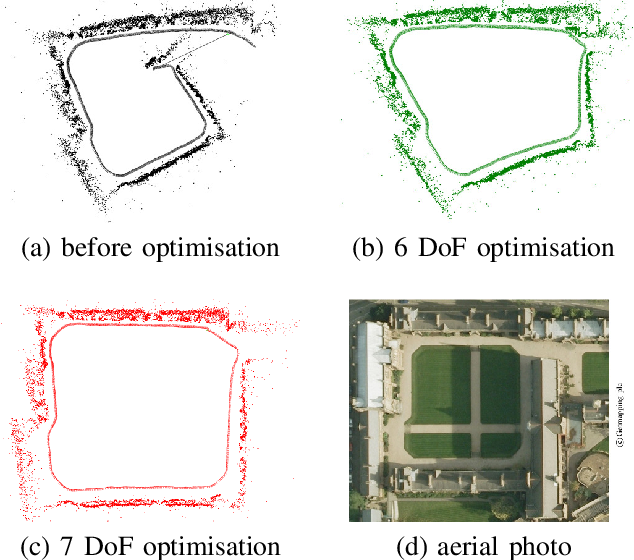
\includegraphics[width=80mm, keepaspectratio]{figures/scale_drift_lsd_slam.png}
    \caption{Scale drift and compensation illustration from \cite{Strasdat2010ScaleDL}}
    \label{fig:scale_drift_lsd_slam}
\end{figure}


\subsubsection{Stereo camera}
A stereo camera is a type of camera with typically two image sensors. Two image sensors mimic the human binocular vision and 
makes depth perception possible. The two cameras are placed relatively close together so there is a high correlation between 
the images taken by these cameras. To find correlations between the two images sufficient details and structure needs to be
present on the images, therefore light conditions affect the performance of depth-sensing. This technique is also called
passive stereo vision.

Active stereo cameras solve this problem employing a projector onboard, that projects a structured light to simplify the 
stereo matching problem. Using this technique the depth sensing performance is less affected by lighting conditions and 
reoccurring patterns will not confuse the matching of the images.

\begin{figure}[!ht]
    \centering
    $\vcenter{\hbox{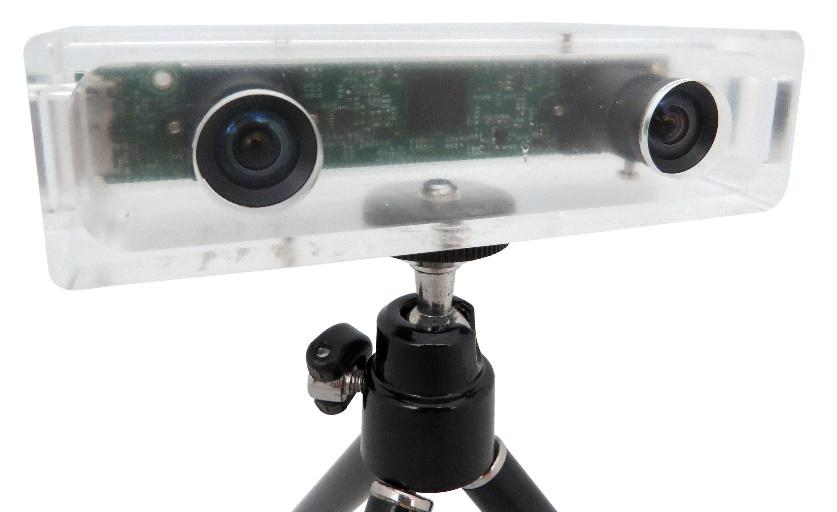
\includegraphics[width=60mm, keepaspectratio]{figures/stereo_camera.jpg}}}$
    $\vcenter{\hbox{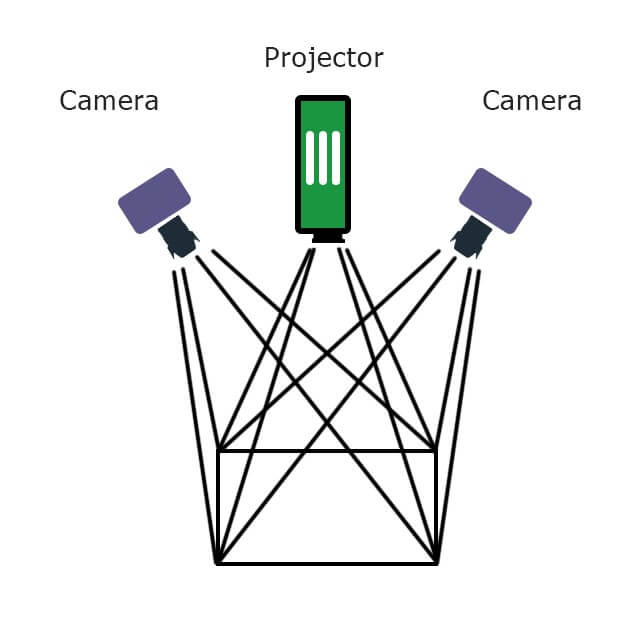
\includegraphics[width=60mm, keepaspectratio]{figures/active_stereo_camera.jpg}}}$
    \caption{Passive stereo camera on the left, concept of active stereo camera on the right }
    \label{fig:stereo_camera}
\end{figure}



\subsubsection{LSD-SLAM}

LSD-SLAM for monocular cameras were proposed in \cite{engel2014lsd} and for stereo or RGB-D cameras in \cite{engel2015large}.
LSD stands for Large-Scale Direct SLAM and it can be seen by the name that it is a direct SLAM algorithm.
The map of the surroundings is created based on keyframes that consists of three fields, a camera image, an inverse depth map
and the variance of the inverse depth map. The solution of the problem proposed by SLAM is divided into three parts, tracking,
depth map estimation and map optimization as seen on figure \ref{fig:lsd_slam_overview}.


\begin{figure}[!ht]
    \centering
    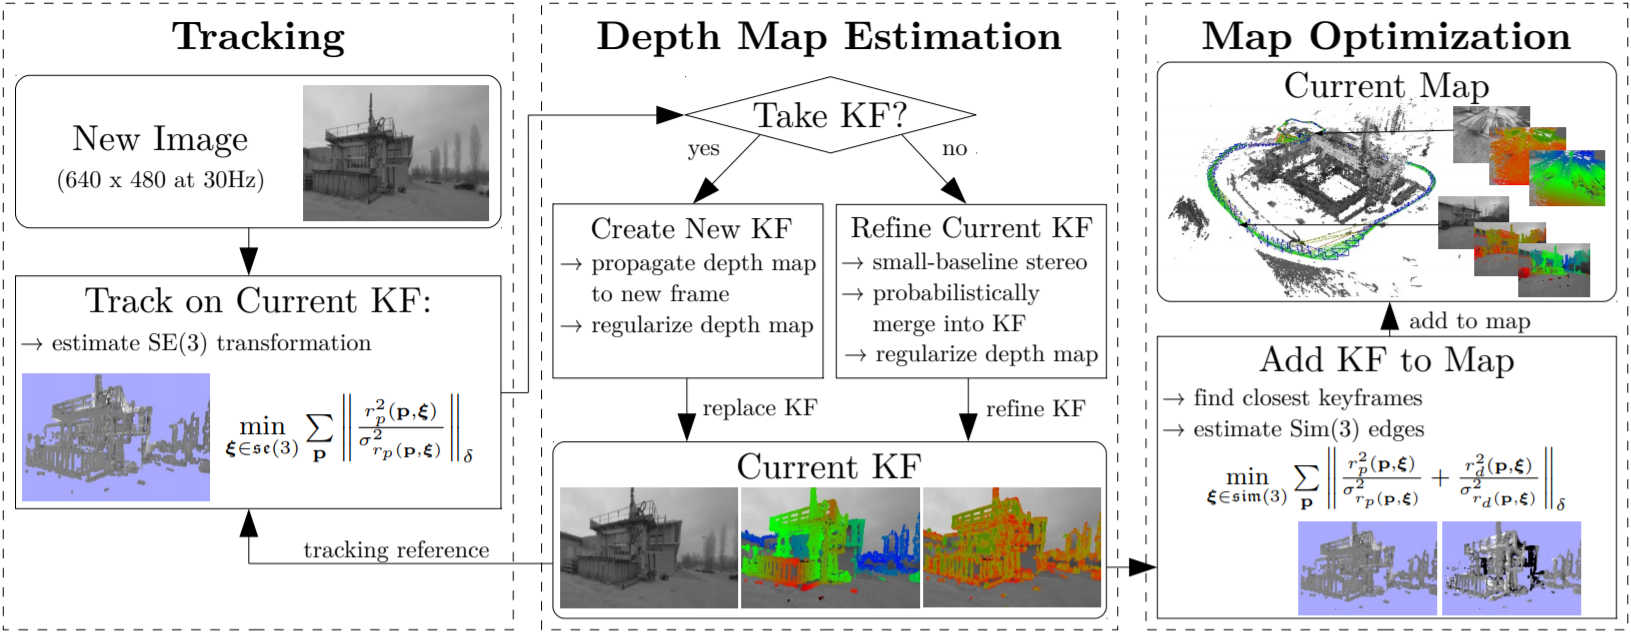
\includegraphics[width=150mm, keepaspectratio]{figures/lsd_slam_overview.png}
    \caption{LSD-SLAM overview of the complete algorithm \cite{engel2014lsd}}
    \label{fig:lsd_slam_overview}
\end{figure}

New images are input during the tracking phase and the position is estimated with respect to the current keyframe from 
previous iteration. The depth map estimation component uses tracked frames to either refine or replace the current keyframe.
If the camera has moved more than a set threshold, a new keyframe is initialized with the combination of current and new 
keyframe. If the tracked keyframe is not taken, then it is used to refine the current keyframe by filtering over many per-pixel,
performing small-baseline stereo comparisons and regularization of the depth map. Once the current keyframe is updated, it is 
built into the global map, by the map optimization.
Keyframes that are close to each other can be detected and closed, this process is called loop-closure. For loop closures and
scale-drift compensation, similarity transform is used. The map is further optimized using using pose graph optimization from 
g2p package.

\subsubsection{ORB-SLAM}
ORB-SLAM is a feature-based SLAM algorithm introduced in \cite{mur2015orb}. The features extracted are represented by ORBs,
therefore the name of the algorithm. ORB-SLAM has three threads that run in parallel: tracking, local mapping and 
loop closing.

The tracking phase is responsible for localizing the camera and to decide when to insert a new keyframe.
The features extracted from the new image are FAST corners, where FAST is a computationally efficient process to find corners
on images. These corners are described using ORB, that is a method to describe FAST corners by a center of mass and
an orientation parameter. This way the place and orientation is known of each feature.The initial pose is estimated using 
a constant velocity model and if the tracking is lost relocation is done instead of pose estimation.
Track local map is a map of keyframes that share a common map point. Finally it is decided if new keyframe is need to be
created.


\begin{figure}[!hb]
    \centering
    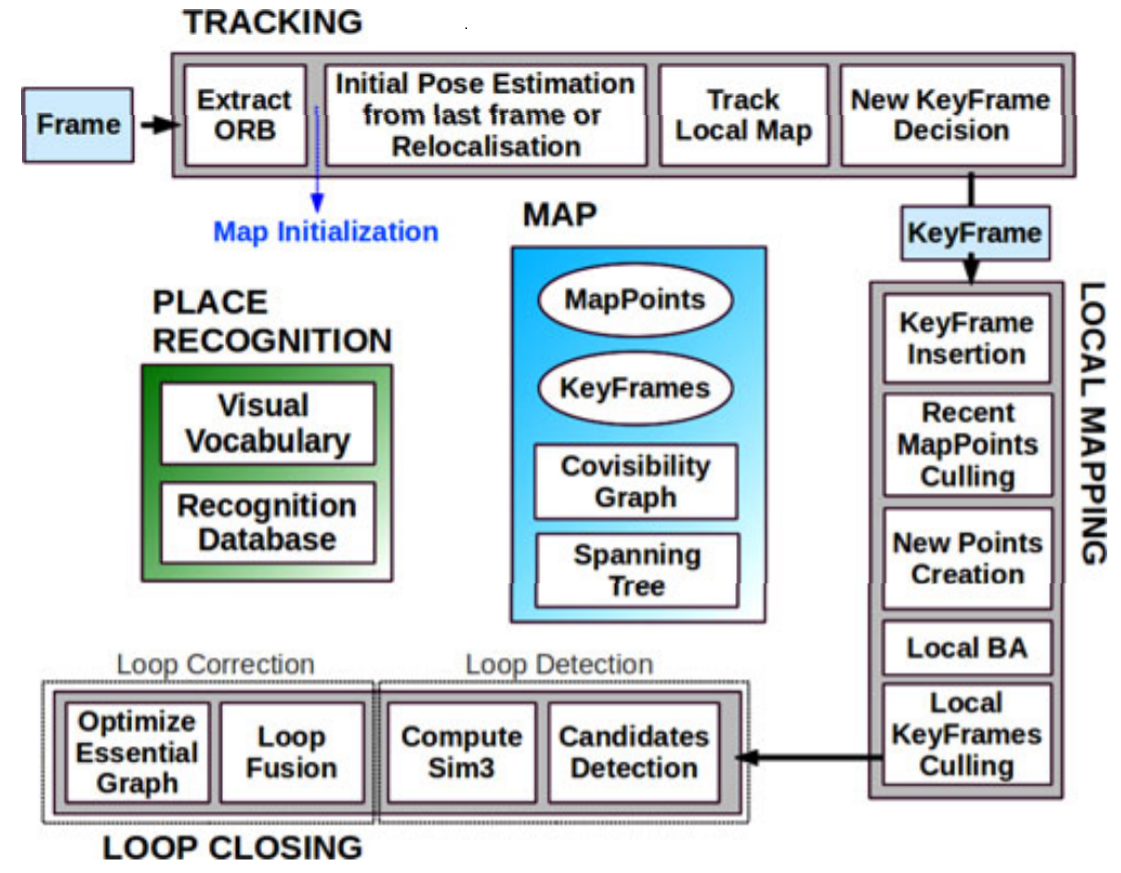
\includegraphics[width=150mm, keepaspectratio]{figures/orb_slam_overview.png}
    \caption{ORB-SLAM overview \cite{mur2015orb}}
    \label{fig:orb_slam_overview}
\end{figure}


In the first step of local mapping the new keyframe is inserted into the co-visibility graph and it is linked keyframe to keyframe
with the most points in common. ORB features from the connected keyframes are used to calculate new map points using triangulation. 
Unmatched ORBs are compared with other unmatched ORBs of other keyframes. Projection error and consistency is checked, then the 
map is projected to the matched keyframes. The new map points need to be validated, by going through a test to increase the 
likelihood that these map points are valid part of the map. In local bundle adjustment step the current keyframe and connected
keyframes through the co-visibility graph are optimized. Finally abundant keyframes get discarded to keep simplicity.

Loop closing is quite effective in ORB-SLAM, because matching ORBs can be done with relatively high confidence. Similarity 
transformation is calculated.

\subsection{Ranging sensor based SLAM}
Cameras are cheap, popular and can be used to create highly detailed maps, but they produce high amounts of data that demands 
high processing capabilities. Sensor based approaches produce lower amount of data that is dependent on the scale, sensors have
a minimum and maximum range they can be used on.

Ultrasonic sensors are easy to use for distance measurements, they are cheap and easy to use, but they suffer from significant
measurement noise, because of background noise and the variability of speed of sound. LIDAR sensors on the other hand 
use light to measure distance, offer more accurate measurements, typically lower form factor, higher resolution and update rates. LIDAR 
sensors are also significantly more expensive than most of ultrasonic sensors and camera based SLAM systems.

A planar laser scanner is a LIDAR sensor that is extended to make distance measurements in 2D. Typically it is used for 
scanning the horizontal plane. Usually the scanning is solved by rotating a LIDAR sensor in 360$^\circ$ while it is 
making measurements evenly distributed on the plane. Planar scanners are good for building floor maps and navigating in indoor 
environments. Some scanners are further extended for 3D scanning.


\subsubsection{3D LIDAR SLAM to improve localization accuracy} \label{lidar_for_localization}

The study of University of California\cite{hening20173d} presents an algorithm that fuses LIDAR, IMU and GPS signals 
to have a more accurate estimation of the absolute position and velocity of a UAV. The LIDAR scanner provides local position
updates using SLAM technique, GPS provides corrections when available and an Internal Navigation System is used as an 
additional input to the Adaptive Extended Kalman filter. The outline of the filter can be seen on figure \ref{fig:haning_filter}.

The 3D LIDAR scanner used is Velodyne VLP-16, that has a vertical field of view of 30$^\circ$ with a vertical resolution 
of 2$^\circ$. On the horizontal axis the resolution is 0.1-0.4$^\circ$ and rotation rate can be adjusted between 5-20Hz.
The sensor weighs 830g according to the company website.

During the experiment an octocopter is used to carry the sensor. Octocopters are stable and can carry high amounts of weight.
The proposed filter is was capable of reducing the GPS drift of 24.3m and LIDAR drift of 7.5m to 3.42m.
This shows that fusing GPS, LIDAR and IMU measurements results in a more accurate position estimate in
GPS-degraded environments. The capabilities of the LIDAR was also tested on an even moon like surface, 
with very few landmarks that can be used by the SLAM algorithm. In this case GPS data is much more 
accurate than LIDAR SLAM, therefore LIDAR data is not used for calculation of position updates.

\begin{figure}[!ht]
    \centering
	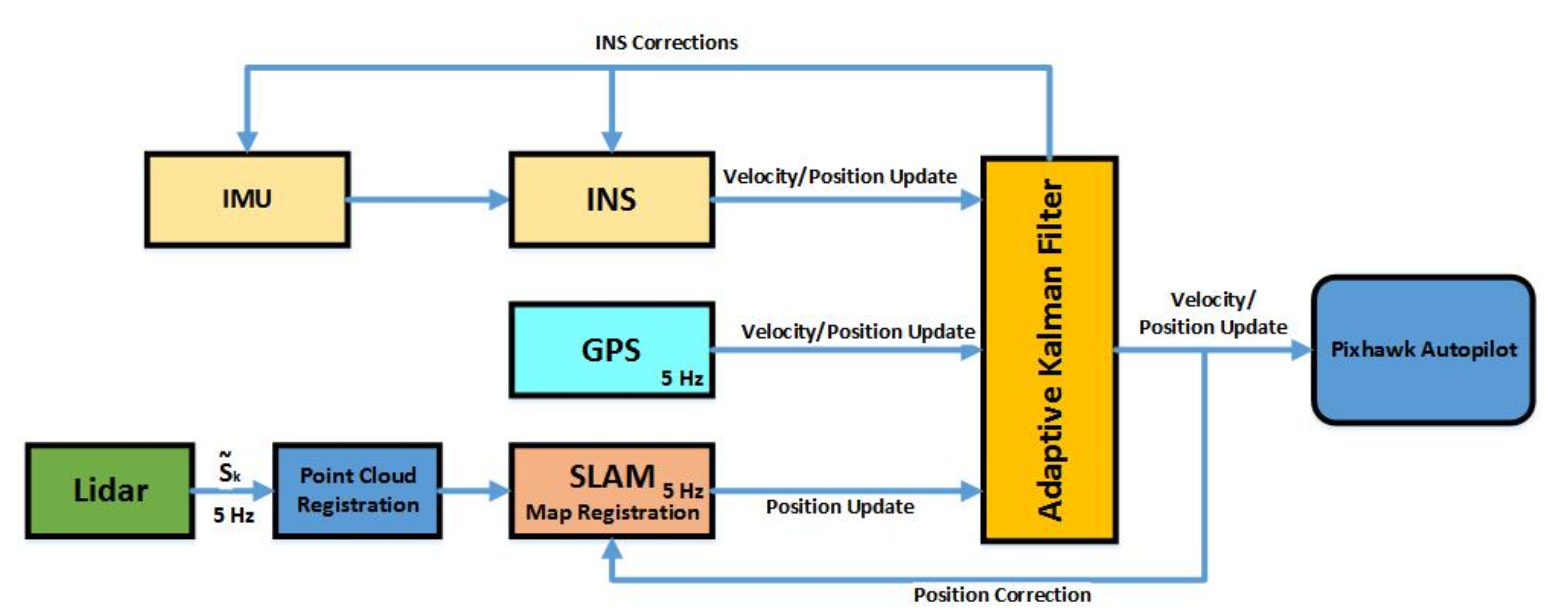
\includegraphics[width=100mm, keepaspectratio]{figures/hening_filter.png}
    \caption{3D LiDAR SLAM Integration with GPS/INS for UAVs in Urban GPS-Degraded Environments \cite{hening20173d} - algorithm overview}
    \label{fig:haning_filter}
\end{figure}

\begin{figure}[!ht]
    \centering
	$\vcenter{\hbox{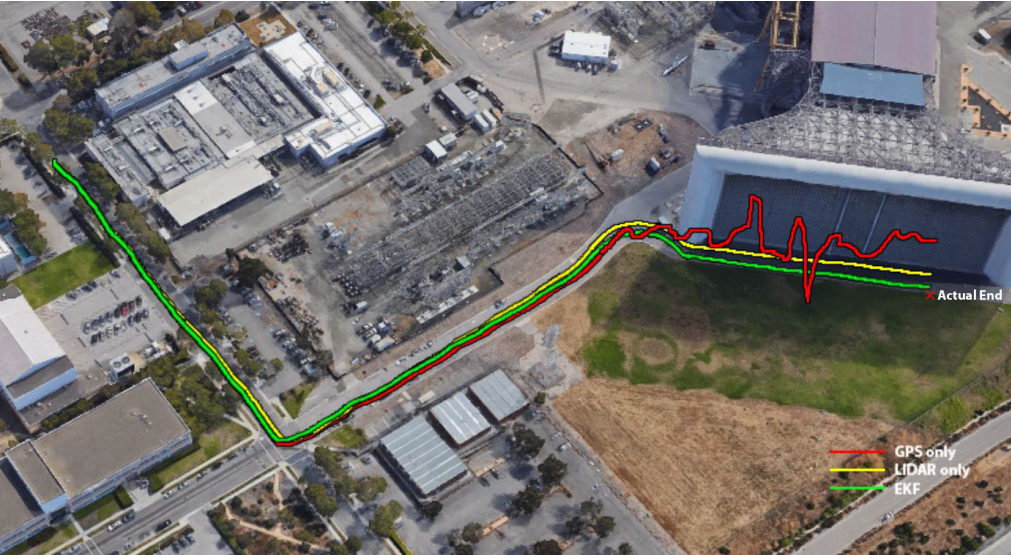
\includegraphics[width=80mm, keepaspectratio]{figures/hening_LIDARvsGPS.png}}}$
	$\vcenter{\hbox{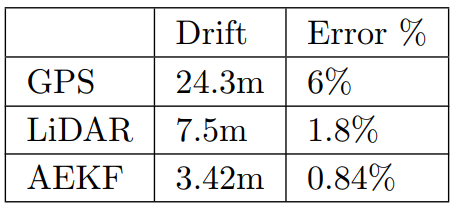
\includegraphics[width=50mm, keepaspectratio]{figures/hening_result.png}}}$
    \caption{GPS, LIDAR and EKF position estimates and position drift after 405 meters\cite{hening20173d}}
    \label{fig:lidar_slam_integration}
\end{figure}


\subsubsection{3D LIDAR SLAM for mapping}
The solution seen in \ref{lidar_for_localization} uses a LIDAR scanner to improve position and velocity data, by fusing the output 
of SLAM algorithm with others. The map created simultaneously is not used in this solution. 3D LIDAR data and SLAM can be also used 
to create highly detailed maps. The paper, presented by David Droeschel and Sven Behnke \cite{droeschel2018efficient}, discusses
an efficient implementation of SLAM with focus on improving online mapping quality.

\begin{figure}[!ht]
    \centering
	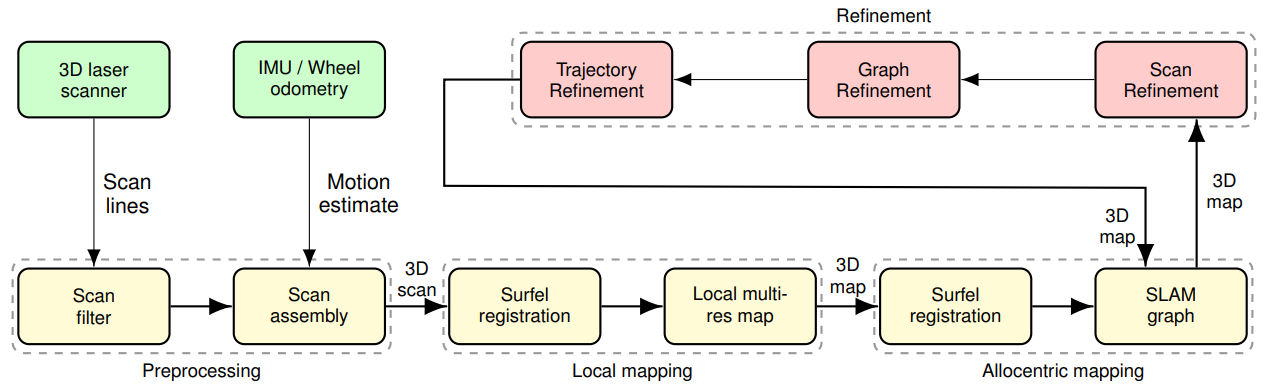
\includegraphics[width=140mm, keepaspectratio]{figures/droeschel_overview.png}
    \caption{Efficient Continuous-time SLAM for 3D LIDAR-based online mapping\cite{droeschel2018efficient} - algorithm overview}
    \label{fig:3d_lidar_mapping_overview}
\end{figure}

\begin{figure}
    \centering
    $\vcenter{\hbox{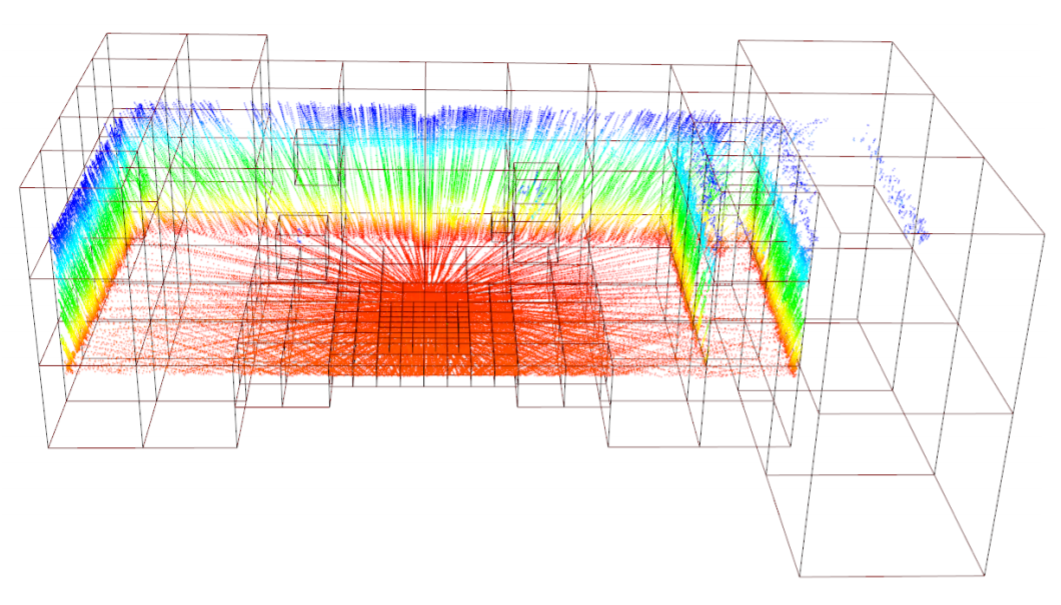
\includegraphics[width=80mm, keepaspectratio]{figures/3d_slam_gridmap.png}}}$
	$\vcenter{\hbox{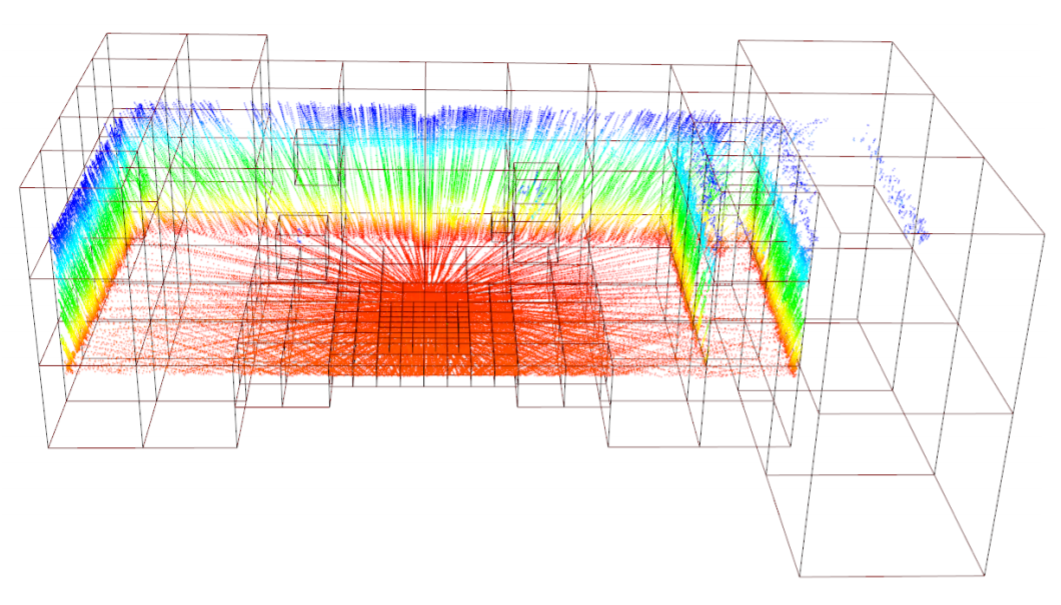
\includegraphics[width=50mm, keepaspectratio]{figures/3d_slam_gridmap.png}}}$
    \caption{Grid-map presented in \cite{droeschel2014local} on the left, ... on the right} 
    \label{fig:3d_lidar_mapping_figures}
\end{figure}

The system first aggregates range measurements into a robot-centric grid-map \cite{droeschel2014local}, that has high resolution
in the close proximity and lower resolution with increasing distance. A grid cell stores the cell's occupancy probability and a
surface element(surfel), that describes the mean of samples and covariance. IMU or odometry measurements are used to account for 
motion of the sensor during acquisition, to compensate rolling shutter artifacts. After the preprocessing step, local maps are 
updated 






\subsection{Cartographer SLAM}
Cartographer is a system developed by Google that provides real-time simultaneous localization and mapping
in 2D and 3D across multiple platforms and sensor configurations. Cartographer is used by Google street view
for internal mapping of building interiors, using a backpack mounted LIDAR scanner.

There officially available SLAM packages in ROS, the two most popular packages are Gmapping and Cartographer.
Gmapping package contains a ROS wrapper for OpenSlam's Gmapping that provides laser based SLAM as a ROS node. 
Gmapping is limited to 2D map building, therefore it is not considered for this project.

\begin{figure}[!ht]
    \centering
	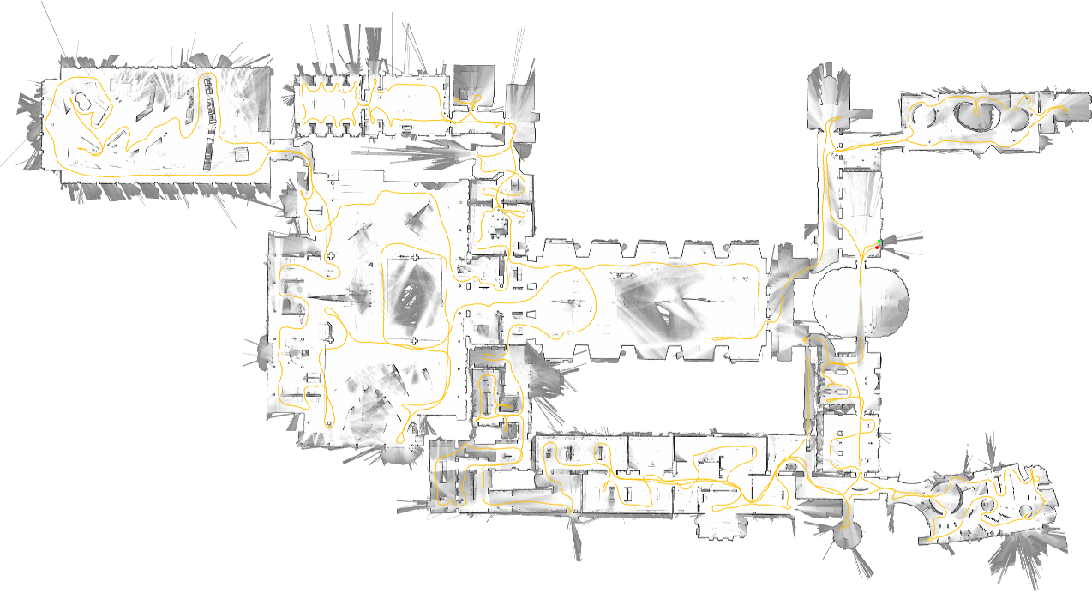
\includegraphics[width=140mm, keepaspectratio]{figures/cartographer_example.png}
    \caption{Cartographer SLAM example\cite{CartographerDocumentation}}
    \label{fig:cartographer_slam_example}
\end{figure}


On the other hand Cartographer ROS package supports both 2D and 3D SLAM and has a great and active community.
The overview of Cartographer is seen on figure \ref{fig:cartographer_slam_overview}. The core components are
sensor inputs, Local SLAM and Global SLAM. On a higher abstraction the job of local SLAM is to build submaps
and the job of global SLAM is to tie submaps the most consistently together.
It is common to build submaps or local maps in SLAM implementations, because building a single map increases 
complexity quadratically, but by using submaps the complexity can be limited to the contents of the submap.

The most important input of Cartographer is the Range Data, depth information coming from LIDAR sensors. 
The data is first pre-filtered, because some measurements are irrelevant the sensor might be directed to
a part of the robot or it can be covered by dust. Some sensors set unsuccessful range measurements to a value
that is significantly higher than the maximum range of the sensor. A bandpass filter is used for pre-filtering,
that keeps the values in a predefined range. The minimum and maximum values need to be set according to 
the sensor specifications. Close objects are very often hit by the LIDAR
measurements and offer more points, however distant objects offer much less points. The Voxel filter 
downsamples raw points where density is higher to reduce computation needed.

Inertial Measurement Units (IMU) provide a direction of gravity vector and a noisy estimation of the robot's
rotation. IMU data has to be provided for 3D SLAM because it greatly reduces complexity of scan matching,
while IMU data is optional for 2D SLAM. Odometry Pose and Fixed Frame Pose are optional inputs of 
Cartographer, that can further reduce complexity.


\begin{figure}[!hb]
    \centering
	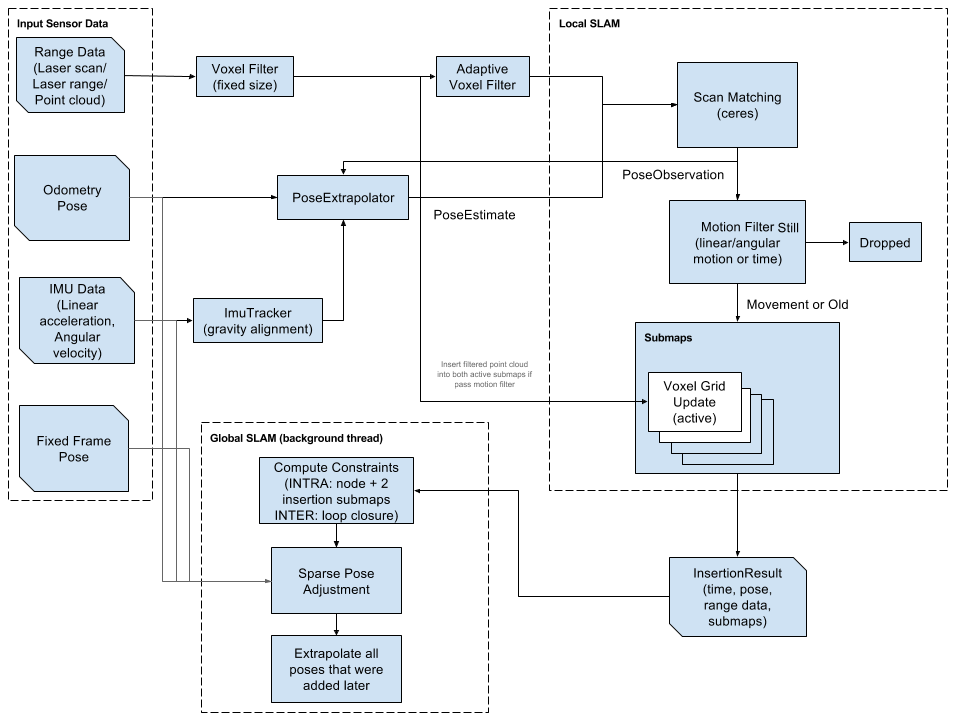
\includegraphics[width=140mm, keepaspectratio]{figures/cartographer_slam.png}
    \caption{Cartographer SLAM overview\cite{CartographerDocumentation}}
    \label{fig:cartographer_slam_overview}
\end{figure}



\section{Similar products available on the market} 

\subsection{Terabee TeraRanger Tower} \label{sect:TerabeeDescription}
TeraBee offers an off-the-shelf solid-state LIDAR system with the purpose of collision avoidance for drones.
In their solution 8 sensors are evenly distributed around the vertical axis with a controller board in 
the middle. TeraRanger's interface is compatible with Pixhawk 4 flight controller board and 
PX4 flight controller software, that makes integration easy into systems based on these.

\begin{figure}[!ht]
    \centering
    $\vcenter{\hbox{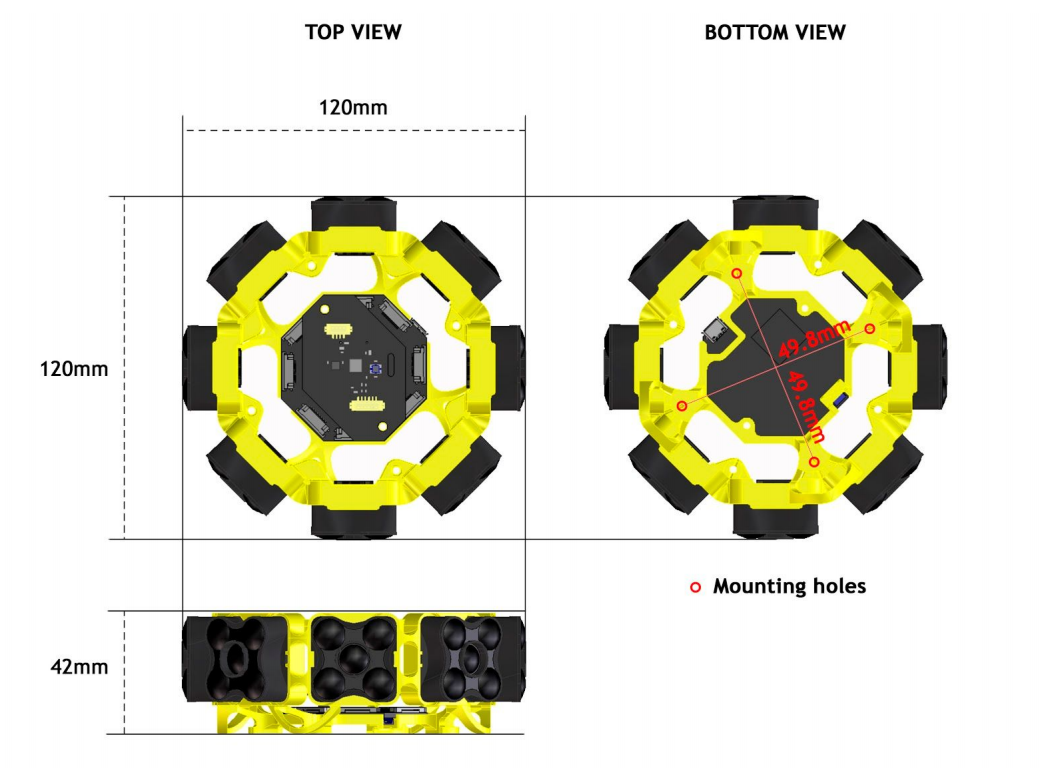
\includegraphics[width=80mm, keepaspectratio]{figures/tera_ranger_tower.png}}}$
    $\vcenter{\hbox{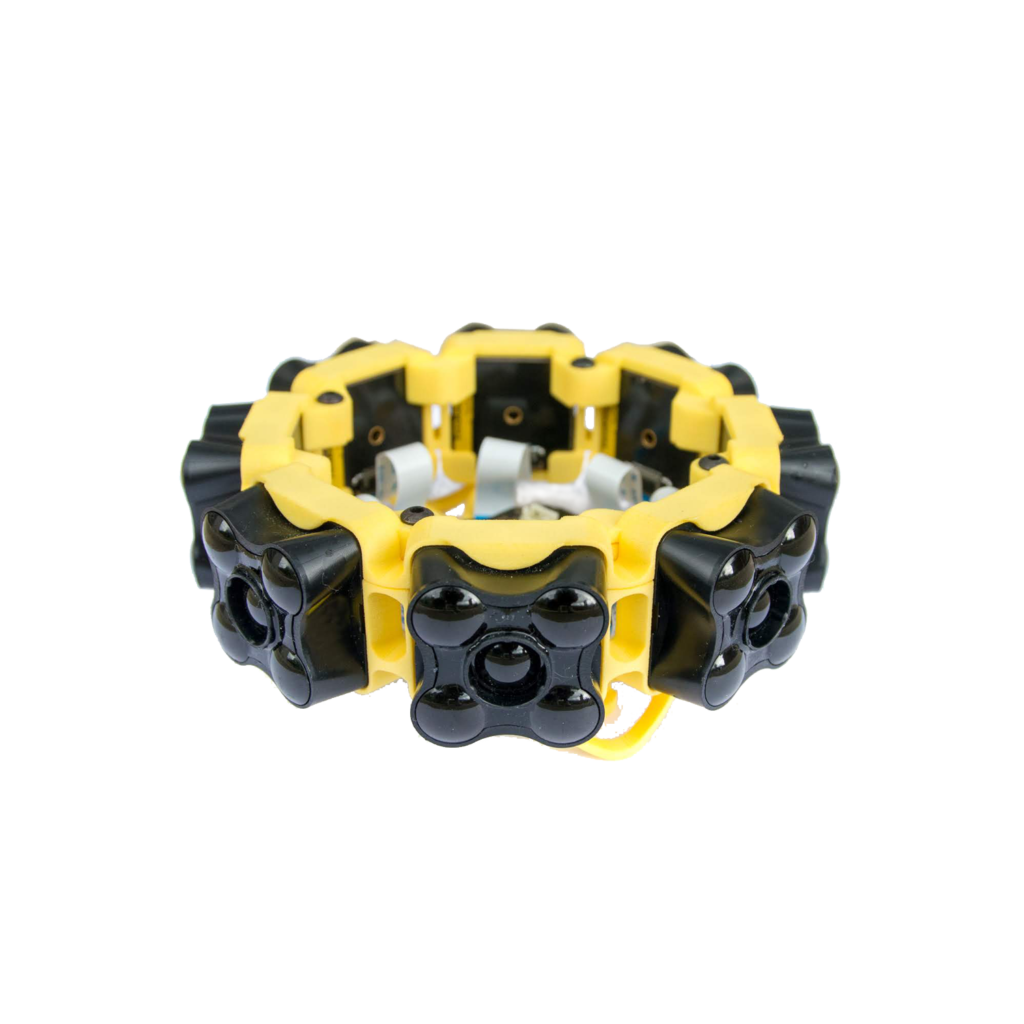
\includegraphics[width=50mm, keepaspectratio]{figures/tera_ranger_tower_2.png}}}$
    \caption{Terabee TeraRanger Tower Evo dimensions}
    \label{fig:teraranger_dimensions}
\end{figure}

Each block of the array is a standalone LIDAR sensor, that can be used separately and supports different
mount configurations. The company offers a long-range and fast-ranging version of these sensors, depending 
on the type an update rate of 320 Hz can be achieved. The fact that system comes with a ROS package and a 
2$^{\circ}$ field of view makes it a potential candidate for indoor mapping and positioning in two dimensions. 
The price of this setup starts from 599 euro\cite{TerabeeTeraRanger}.

\begin{table}[ht]
	\footnotesize
	\centering
	\begin{tabular}{ l c c }
		\toprule
		                & Long-range                                & Fast-ranging \\
		\midrule
		Range           & 0.5m up to 60m                            & 0.75m up to 8m \\
		Update rate     & 120Hz/sensor                              & 320Hz/sensor\\
		Field of View   & 2$^{\circ}$                               & 2$^{\circ}$\\
		Accuracy        & $\pm 4cm$ in the first 14m, 1.5\% above   & $\pm 12cm$\\
		\bottomrule
	\end{tabular}
	\caption{TeraRanger Tower Evo specifications}
	\label{tab:tera_ranger_features}
\end{table}

Terabee provides a tutorial video on their website\cite{TerabeeTeraRanger} how to connect the 
sensor array to a UAV that uses Pixhawk 4 flight controller and the process of configuration 
in two different GCS programs. I have learned that PX4 flight stack supports lidar measurements
for obstacle avoidance and it can be configured from a GCS program. It seems a reasonable choice 
to integrate this feature into such product.

\subsection{Crazyflie Multi-ranger deck}
The company Bitcraze has developed a mini quadcopter mainly for educational purposes. The current version is
called Crazyflie 2.1 and measures only 92x92mm with a height of 29mm and a weighs 27g.
Extra sensors and peripherals can be attached to the top of the quadcopter using extension boards.

The extension board called Multi-ranger deck has 5 VL53L1X sensors by STMicroelectronics facing forwards, 
backwards, left, right and up. This project is similar to the product of Terabee described in \ref{sect:TerabeeDescription}, 
but in a smaller size factor and with significantly lower weight.

An introduction video can be found on the product website \cite{BitcrazeMultirangerDeck}, where 
a SLAM algorithm is used to create a map and localize the drone. This serves as a proof of concept,
that static VL53L1X sensors can be used for mapping and positioning in two dimensions. The company provided 
no information of the SLAM algorithm used or from the quality of the map.

\begin{figure}[!ht]
    \centering
    $\vcenter{\hbox{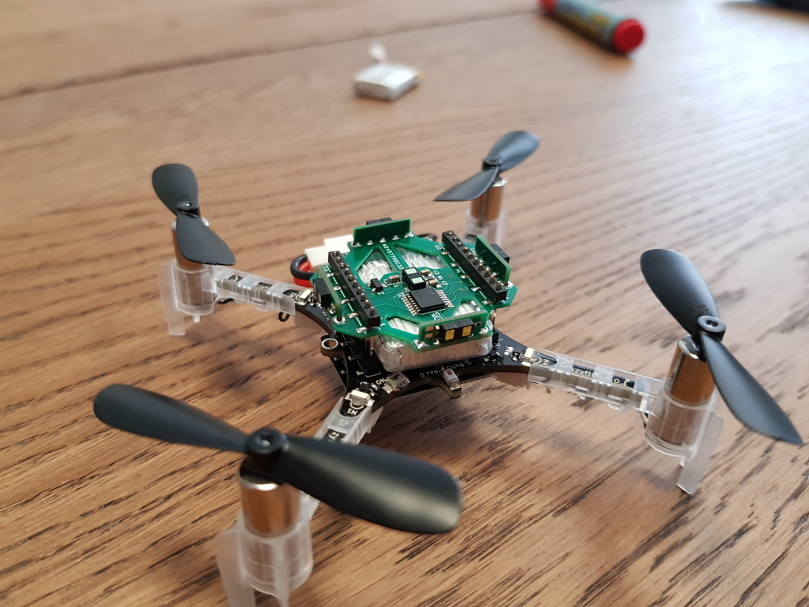
\includegraphics[width=60mm, keepaspectratio]{figures/multiranger_deck.jpg}}}$
    $\vcenter{\hbox{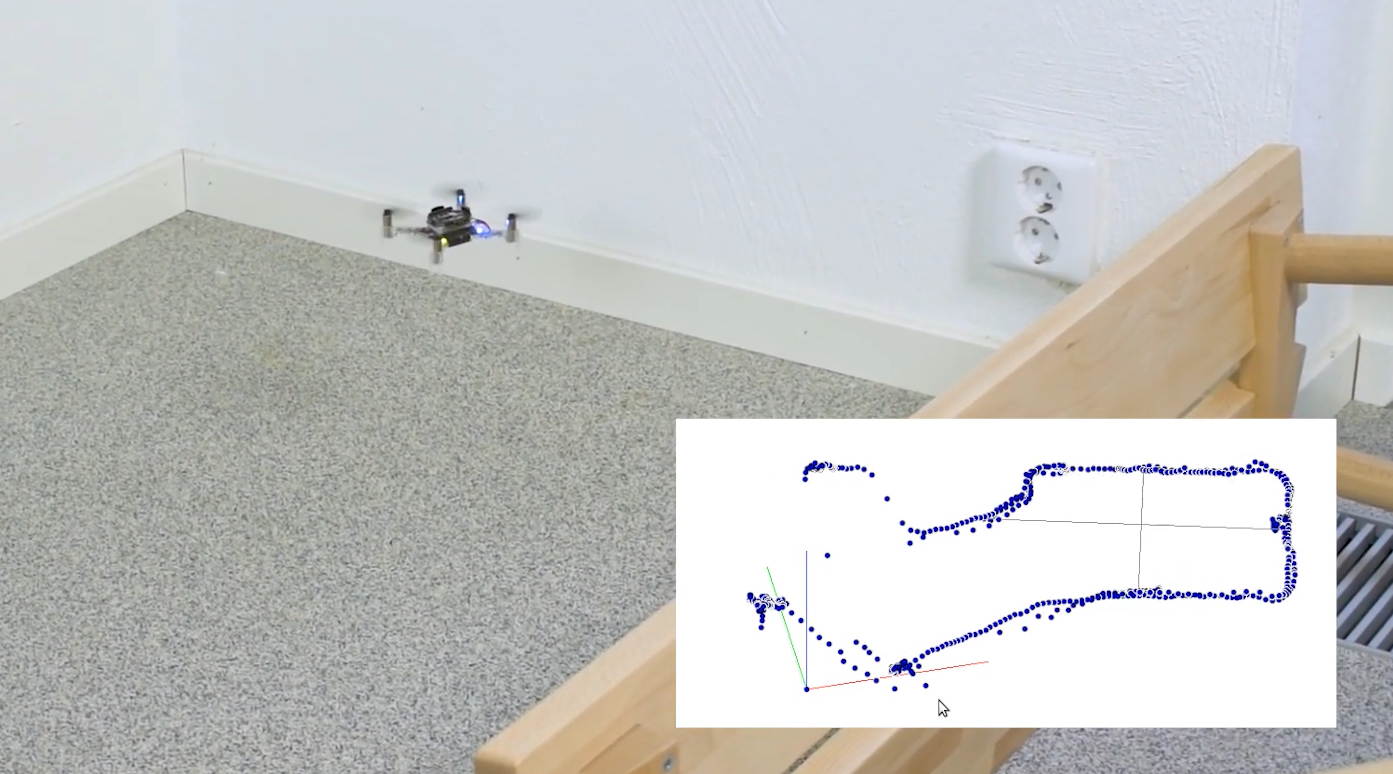
\includegraphics[width=80mm, keepaspectratio]{figures/multiranger_slam.png}}}$
    \caption{Crazyflie Multi-ranger deck, SLAM example project}
    \label{fig:crazyflie_multiranger}
\end{figure}

